\documentclass[twocolumn]{article}
\usepackage[spanish]{babel}
\usepackage[utf8]{inputenc}
\usepackage{amssymb}
\usepackage{graphicx}
\usepackage{verbatim}
\usepackage{algorithmic}
\usepackage{enumitem}
\setlist{nolistsep}
\usepackage{fancyvrb}



\author{
Nombre:....................................... \\
    Departamento de Informática y Sistemas \\
    Universidad EAFIT \\
}
\title{
    Estructuras de Datos 2 - ST0247 \\
    Examen Parcial 2
}
\date{
    Octubre 26 de 2017
}

\begin{document}
\vspace{-5cm}
\maketitle


\section*{Criterios de calificación}

\begin{itemize}
\item Selección múltiple con única respuesta
\begin{itemize}
\item Respuesta correcta: 100\%
\item Respuesta incorrecta: 0\%
\end{itemize}

\item Completar código
\begin{itemize}
\item Respuesta correcta 100\%
\item Respuesta incorrecta o vacía 0\%
\end{itemize}
\end{itemize}

%\vspace{1cm}

\textbf{NOTAS IMPORTANTES:}
\begin{itemize}
	\item Responda en la hoja de PREGUNTAS
	\item Marque la hoja de PREGUNTAS
\end{itemize}

\section{Prog. Dinámica 30\%}
La distancia de Levenshtein es el número mínimo de operaciones requeridas para transformar una cadena de caracteres en otra. Se entiende por operación, una inserción, eliminación o la sustitución de un carácter. Es útil en programas que determinan cuán similares son dos cadenas de caracteres, como es el caso de los correctores de ortografía. Como un ejemplo, la distancia de Levenshtein entre ``casa'' y ``calle'' es de $3$ porque se necesitan al menos tres ediciones elementales para cambiar uno en el otro:

\begin{enumerate}
   \item casa $\rightarrow$ cala (sustitución de 's' por 'l')
  \item  cala $\rightarrow$ calla (inserción de 'l' entre 'l' y 'a')
   \item calla $\rightarrow$ calle (sustitución de 'a' por 'e')
\end{enumerate}


A continuación está una implementación del algoritmo en Java:

{\small
\begin{verbatim}
int minimum(int a, int b, int c) {                            
  return Math.min(Math.min(a, b), c);                                      
}                                                                            
                                                                                
int Levenshtein(String lhs, String rhs) {      
  int[][] distance = new int[lhs.length() + 1]
                            [rhs.length() + 1];                                   
  for (int i = 0; i <= lhs.length(); i++)                                 
    distance[i][0] = i;                                                  
  for (int j = 1; j <= rhs.length(); j++)                                 
    distance[0][j] = j;                                                                     
  for (int i = 1; i <= lhs.length(); i++)                                 
    for (int j = 1; j <= rhs.length(); j++)                             
     distance[i][j] = minimum(                                        
      distance[i - 1][j] + 1,                                  
      distance[i][j - 1] + 1,                                  
      distance[i - 1][j - 1] + 
      ((lhs.charAt(i - 1) == 
        rhs.charAt(j - 1)) ? 0 : 1));                                                           
  return distance[lhs.length()][rhs.length()];                          
}                                                                            
\end{verbatim}
}


En Java, el operador incógnita (?) funciona de la siguiente forma: Si \texttt{algo} es verdadero, entonces retorna un \texttt{valor},
de lo contrario retorna \texttt{otro valor}, así:
\texttt{algo ? un valor : otro valor}.


(15 \%) Complete la siguiente tabla, siguiendo el algoritmo de programación dinámica de la distancia de Levenshtein:\\

\begin{tabular}{| l  | l  | l  | l  | l  | l  | l |}
\hline
  & & c & a & l & l & e \\
 \hline
  & &  &  &  &  &  \\
  \hline
c & &  &  &  &  &  \\
\hline
a & &  &  &  &  &  \\
\hline
s & &  &  &  &  &  \\
\hline
a & &  &  &  &  &  \\
\hline
\end{tabular}

%  	  	c 	a 	l 	l 	e
%   	0 	1 	2 	3 	4 	5
% c 	1 	0 	1 	2 	3 	4
% a 	2 	1 	0 	1 	2 	3
% s 	3 	2 	1 	1 	2 	3
% a 	4 	3 	2 	2 	2 	3

(15 \%) Complete la siguiente tabla, siguiendo el algoritmo de programación dinámica de la distancia de Levenshtein, para encontrar
la distancia entre madre y mama:\\

\begin{tabular}{| l  | l  | l  | l  | l  | l  | l |}
\hline
  & & m & a & d & r & e \\
 \hline
  & &  &  &  &  &  \\
  \hline
m & &  &  &  &  &  \\
\hline
a & &  &  &  &  &  \\
\hline
m & &  &  &  &  &  \\
\hline
a & &  &  &  &  &  \\
\hline
\end{tabular}


\section{Prog. Dinámica 20\%}
Considere un grafo dirigido representado por la siguiente matriz de adyacencia:

\begin{tabular}{|l|l|l|l|l|}
\hline
& 0 & 1 & 2 & 3 \\
\hline
0 & 0 & 1 & 15 & 6 \\
\hline
1 & 2 & 0 & 7 & 3 \\
\hline
2 & 9 & 6 & 0 & 12 \\
\hline
3 & 10 & 4 & 8 & 0 \\
\hline
\end{tabular}

3.1 (10\%) Complete, por favor, la siguiente tabla, usando el algoritmo de programación dinámica del agente viajero, también conocido como el
\textbf{algoritmo de Held-Karp}. El algoritmo funciona de la siguiente forma.
Primero, calcula todos los subconjuntos del conjunto de vértices sin incluir el primer vértice (es decir, el vértice $0$).
Después, crea una tabla en la que se coloca cuál es el costo del camino más
corto para ir desde $0$ hasta cada vértice pasando por los vértices del conjunto vacío.
Después, se hace la misma pregunta pero esta vez pasando por los vértices de un conjunto de un elemento.
Posteriormente, la misma pregunta pero pasando por los vértices de un conjunto de dos elementos.
Y así sucesivamente, hasta poder responder la pregunta de cuál es el costo mínimo de un camino que inicia
en el vértice $0$ y termina en el vértice $0$ y pasa por todos los vértices
del conjunto de vértices quitando el vértice $0$. Para cada paso, utiliza los valores
calculados previamente en la tabla. Para el primer paso utiliza solamente la información
que hay en la matriz de adyacencia que representa el grafo.

En la tabla, la primera línea significa, ¿cuál es el costo para ir desde $0$ hasta $1$ sin pasar por ningún otro vértice (es decir, $\emptyset$) y quién el antecesor visitado antes de ir al vértice $1$. \\

\begin{tabular}{|l|l|l|}
\hline
& Costo & Antecesor \\
\hline
$[1,\emptyset]$ & 1 & 0 \\
\hline
$[2,\emptyset]$ & &  \\
\hline
$[3,\emptyset]$ & &  \\
\hline
$[2,\{1\}]$ & &  \\
\hline
$[3,\{1\}]$ & &  \\
\hline
$[1,\{2\}]$ & &  \\
\hline
$[3,\{2\}]$ & &  \\
\hline
$[1,\{3\}]$ & &  \\
\hline
$[2,\{3\}]$ & &  \\
\hline
$[3,\{1,2\}]$ & &  \\
\hline
$[1,\{2,3\}]$ & &  \\
\hline
$[2,\{1,3\}]$ & &  \\
\hline
$[0,\{1,2,3\}]$ & &  \\
\hline
\end{tabular}

3.2 (10\%) ¿Cuál es el camino con la solución y el costo (también conocido como el peso o la distancia) total del camino?\\

Camino: \_\_\_ $\rightarrow$ \_\_\_ $\rightarrow$ \_\_\_ $\rightarrow$ \_\_\_ $\rightarrow$ \_\_\_ \ \ Costo: \_\_\_


\section{Algo. voraces 30\%}
El algoritmo de Dijkstra sirve para encontrar el camino más corto
de un vértice a todos los demás de un grafo. A continuación una
implementación en Java.

{\small
\begin{verbatim}
int minVertex (int [] dist, boolean [] v) {
 int x = Integer.MAX_VALUE; //Infinity
 int y = -1;   
 for (int i=0; i<dist.length; i++) 
  if (!v[i] && dist[i]<x) 
     y=i; x=dist[i];
 return y;
}
      
int [] dijsktra(Graph dg, int source) {
  int [] dist = new int [dg.size()]; 
  int [] pred = new int [dg.size()]; 
  boolean [] visited = new boolean [dg.size()]; 
  for (int i=0; i<dist.length; i++) 
    dist[i] = Integer.MAX_VALUE; 
  dist[source] = 0;
  for (int i=0; i<dist.length; i++) {
    int next = minVertex (dist, visited);
    visited[next] = true;
    ArrayList<Integer> n =
        dg.getSuccessors (next); 
    for (int j=0; j<n.size(); j++) {
      int v = n.get(j);
      int d = dist[next] + 
          dg.getWeight(next,v);
      if (dist[v] > d) {
        dist[v] = d;
        pred[v] = next;
      }}}
  return pred;  
}
\end{verbatim}
}

Considere el siguiente grafo:

\begin{center}
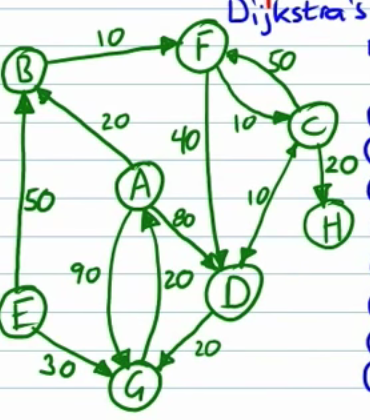
\includegraphics[scale=0.3]{dij.png}
\end{center}

4.1 (20 \%) Complete, por favor, la siguiente tabla, usando
el algoritmo de Dijkstra para encontrar el camino más corto
del punto A a todos los demás. En la tabla, la palabra ``Vi'' significa ``Visitados''.

{\footnotesize
\begin{center}
\begin{tabular}{| c | c | c | c | c | c | c | c | c |}
\hline
Paso  & Vi & B & C & D & E & F & G & H \\
\hline
1 &  A  & $20$,A  & $\infty$  & $80$, A  & $\infty$   & $\infty$  & $90$, A  & $\infty$  \\
\hline
2 &  B  & $20$,A  &  $\infty$  & $80$, A  & $\infty$  & $30$,B  & $90$,A   & $\infty$  \\
\hline
3 &  F &   &   &   &   &   &   &   \\
\hline
4 &   &   &   &   &   &   &   &   \\
\hline
5 &   &   &   &   &   &   &   &   \\
\hline
6 &   &   &   &   &   &   &   &   \\
\hline
7 &   &   &   &   &   &   &   &   \\ 
\hline
8 &   &   &   &   &   &   &   &   \\ 
\hline
\end{tabular}
\end{center}
}

4.2 (10 \%) ¿Cuál es el camino más corto de A a G?\\

  \_\_\_\_\_\_\_\_\_\_\_\_\_\_\_\_\_\_\_\_
\\
\\

\section{Recorridos de grafos 20\%}

Para el grafo siguiente, complete la salida.

\begin{center}
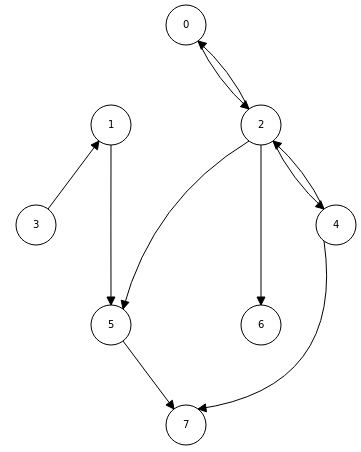
\includegraphics[scale=0.5]{grafin.png}
\end{center}

Complete el orden en que se recorren los nodos usando \textbf{búsqueda en amplitud} (en Inglés BFS) a partir de cada nodo. Si hay varias opciones de recorrer el grafo con BFS, elija siempre el vértice más pequeño.\\


\noindent
$0 \rightarrow$\\
$1 \rightarrow 5 \rightarrow  7$\\
$2 \rightarrow$\\
$3 \rightarrow$\\
$4 \rightarrow$\\
$5 \rightarrow$\\
$6 \rightarrow$\\
$7 \rightarrow$\\




\end{document}
